\documentclass{article}
\usepackage[a4paper, margin=2cm]{geometry}
\usepackage{xcolor}
\usepackage{xspace}
\usepackage{booktabs}
\usepackage{dsfont}
\usepackage{footmisc}
\usepackage{marvosym}
\usepackage{amsmath}
\usepackage{hyperref}
\usepackage[capitalise,noabbrev]{cleveref}
\usepackage{tabularx}
\usepackage{listings}
\usepackage{multirow}
\usepackage{pgfplots}
\pgfplotsset{compat=newest}

\usepgfplotslibrary{groupplots}
\pgfplotsset{every axis/.style={scale only axis}}

\pgfplotsset{
  % Mark repeat, but the last mark is always drawn
  mark repeat*/.style={
    scatter,
    scatter src=x,
    scatter/@pre marker code/.code={
      \pgfmathtruncatemacro\usemark{
        or(mod(\coordindex,#1)==0, (\coordindex==(\numcoords-1))
      }
      \ifnum\usemark=0
        \pgfplotsset{mark=none}
      \fi
    },
    scatter/@post marker code/.code={}
  },
  major grid style={thin,dotted},
  minor grid style={thin,dotted},
  ymajorgrids,
  yminorgrids,
  every axis/.append style={
    line width=0.7pt,
    tick style={
      line cap=round,
      thin,
      major tick length=4pt,
      minor tick length=2pt,
    },
  },
  legend cell align=left,
  legend style={
    line width=0.7pt,
    /tikz/every even column/.append style={column sep=3mm,black},
    /tikz/every odd column/.append style={black},
  },
  % move title closer
  legend style={font=\small},
  title style={yshift=-2pt},
  % less space on left and right
  enlarge x limits=0.04,
  every tick label/.append style={font=\footnotesize},
  every axis label/.append style={font=\small},
  every axis y label/.append style={yshift=-1ex},
  /pgf/number format/1000 sep={},
  axis lines*=left,
  xlabel near ticks,
  ylabel near ticks,
  axis lines*=left,
  label style={font=\footnotesize},       
  tick label style={font=\footnotesize},
}

\title{MPHF plot}
\date{}
\begin{document}
\definecolor{veryLightGrey}{HTML}{F2F2F2}
\definecolor{colorBmz}{HTML}{377EB8}
\definecolor{colorBdz}{HTML}{E41A1C}
\definecolor{colorFch}{HTML}{444444}
\definecolor{colorChd}{HTML}{000000}
\definecolor{colorChm}{HTML}{FF7F00}
\definecolor{colorHeterogeneous}{HTML}{4DAF4A}
\definecolor{colorPthash}{HTML}{984EA3}
\definecolor{colorRecSplit}{HTML}{A65628}
\definecolor{colorBbhash}{HTML}{F781BF}
\definecolor{lightGrey}{HTML}{DDDDDD}
\definecolor{colorSimdRecSplit}{HTML}{444444}
\definecolor{colorChd}{HTML}{377EB8}
\definecolor{colorRustFmph}{HTML}{A65628}
\definecolor{colorRustFmphGo}{HTML}{A65628}
\definecolor{colorRustPHast}{HTML}{FF5733}
\definecolor{colorSicHash}{HTML}{4DAF4A}
\definecolor{colorShockHash}{HTML}{F8BA01}

% IMPORT-DATA competitorNames _competitorNames.txt
% IMPORT-DATA pareto pareto-zoomed.txt
% SQL DELETE FROM pareto WHERE threads != 1 OR loadFactor != 1.0

\begin{figure*}[t]

\centering
    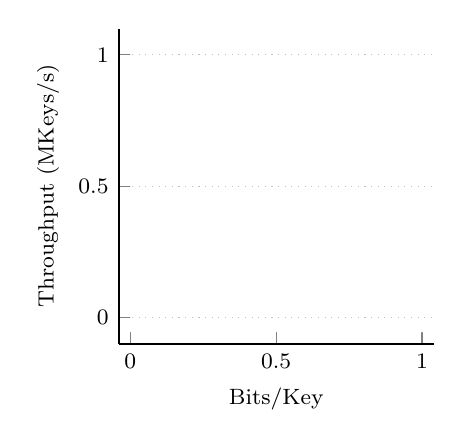
\begin{tikzpicture}
        \begin{axis}[
            xlabel={Bits/Key},
            ylabel={Throughput (MKeys/s)},
            legend to name=paretoLegend,
            legend columns=2,
            width=4cm,
            height=4cm,
          ]
          %% MULTIPLOT(name|ptitle|attr)
          %% SELECT
          %%    bitsPerElement as x,
          %%    0.001*N/constructionTimeMilliseconds as y,
          %%    store_attr || IIF(name LIKE "%PTHash" OR name LIKE "%SicHash" OR name LIKE "ShockHash%", ",mark repeat*=4", "") as attr,
          %%    store_name as ptitle,
          %%    MULTIPLOT
          %% FROM pareto scatterplot
          %% JOIN competitorNames ON name = store_code
          %% WHERE NOT EXISTS (SELECT * FROM pareto d
          %%           WHERE scatterplot.name = d.name
          %%                    AND d.bitsPerElement <= scatterplot.bitsPerElement
          %%                    AND d.constructionTimeMilliseconds <= scatterplot.constructionTimeMilliseconds
          %%                    AND (d.bitsPerElement < scatterplot.bitsPerElement
          %%                        OR d.constructionTimeMilliseconds < scatterplot.constructionTimeMilliseconds))
          %% ORDER BY store_name,x,y

        \end{axis}
    \end{tikzpicture}
    \begin{tikzpicture}
        \begin{axis}[
            xlabel={Bits/Key},
            xmax=1.8,
            ymode=log,
            width=4cm,
            height=4cm,
          ]
          %% MULTIPLOT(name|ptitle|attr)
          %% SELECT
          %%    bitsPerElement as x,
          %%    0.001*N/constructionTimeMilliseconds as y,
          %%    store_attr || IIF(name LIKE "%PTHash" OR name LIKE "%SicHash", ",mark repeat*=4", "") as attr,
          %%    store_name as ptitle,
          %%    MULTIPLOT
          %% FROM pareto scatterplot
          %% JOIN competitorNames ON name = store_code
          %% WHERE NOT EXISTS (SELECT * FROM pareto d
          %%           WHERE scatterplot.name = d.name
          %%                    AND d.bitsPerElement <= scatterplot.bitsPerElement
          %%                    AND d.constructionTimeMilliseconds <= scatterplot.constructionTimeMilliseconds
          %%                    AND (d.bitsPerElement < scatterplot.bitsPerElement
          %%                        OR d.constructionTimeMilliseconds < scatterplot.constructionTimeMilliseconds))
          %% ORDER BY store_name,x,y

          \legend{};
        \end{axis}
    \end{tikzpicture}

    \begin{tikzpicture}
        \ref*{paretoLegend}
    \end{tikzpicture}
    \caption{Space usage vs construction throughput for $N=500 000$ objects ($10$ Million in paper).}
\end{figure*}

\end{document}

